\chapter{Ellipse fitting formulae}
% \markboth{}{Appendix A}
\label{app:ellipse_formulae}

The ellipse fit to obtain the statistical uncertainties on the shift and stretch \acfp{FF} is implemented following the procedure suggested in \Refn{\cite{FitEllipse}}. The fit returns the set of parameters \(\{A,B,C,D,E,F\}\) that parametrise the conic:
\begin{equation*}
    F(x,y) = Ax^2 + Bxy + Cy^2 + Dx + Ey + F = 0
\end{equation*}
with \(B^2 - 4AC < 0\) for ellipses. The variables \(x,y\) shown are general, but in the case of \acp{FF} they represent the shift and stretch parameters, respectively.
\begin{equation}
    \frac{((x-x_0)\cos\theta + (y-y_0)\sin\theta)^2}{a^2} + \frac{((x-x_0)\sin\theta - (y-y_0)\cos\theta)^2}{b^2} = 1,
\end{equation}
it is possible to extract the ellipse center \((x_0, y_0)\), its tilt angle \(\theta\) and its semi-major and semi-minor axis, \(a\) and \(b\), respectively. Then, the desired uncertainties, and the correlation between \(x\) and \(y\) can be extracted using the following relations (see \Fig{\ref{fig:ellipse_formulae:ellipse}}):
\begin{gather}
    \sigma_x = \sqrt{a^2 \cos^2\theta + b^2 \sin^2\theta}\\
    \sigma_y = \sqrt{a^2 \sin^2\theta + b^2 \cos^2\theta}\\
    \rho = \tan(2\theta) \frac{\sigma_{x}^2-\sigma_{y}^2}{2\sigma_{x}\sigma_{y}}.
\end{gather}

\begin{figure}[ht!]
    \centering
    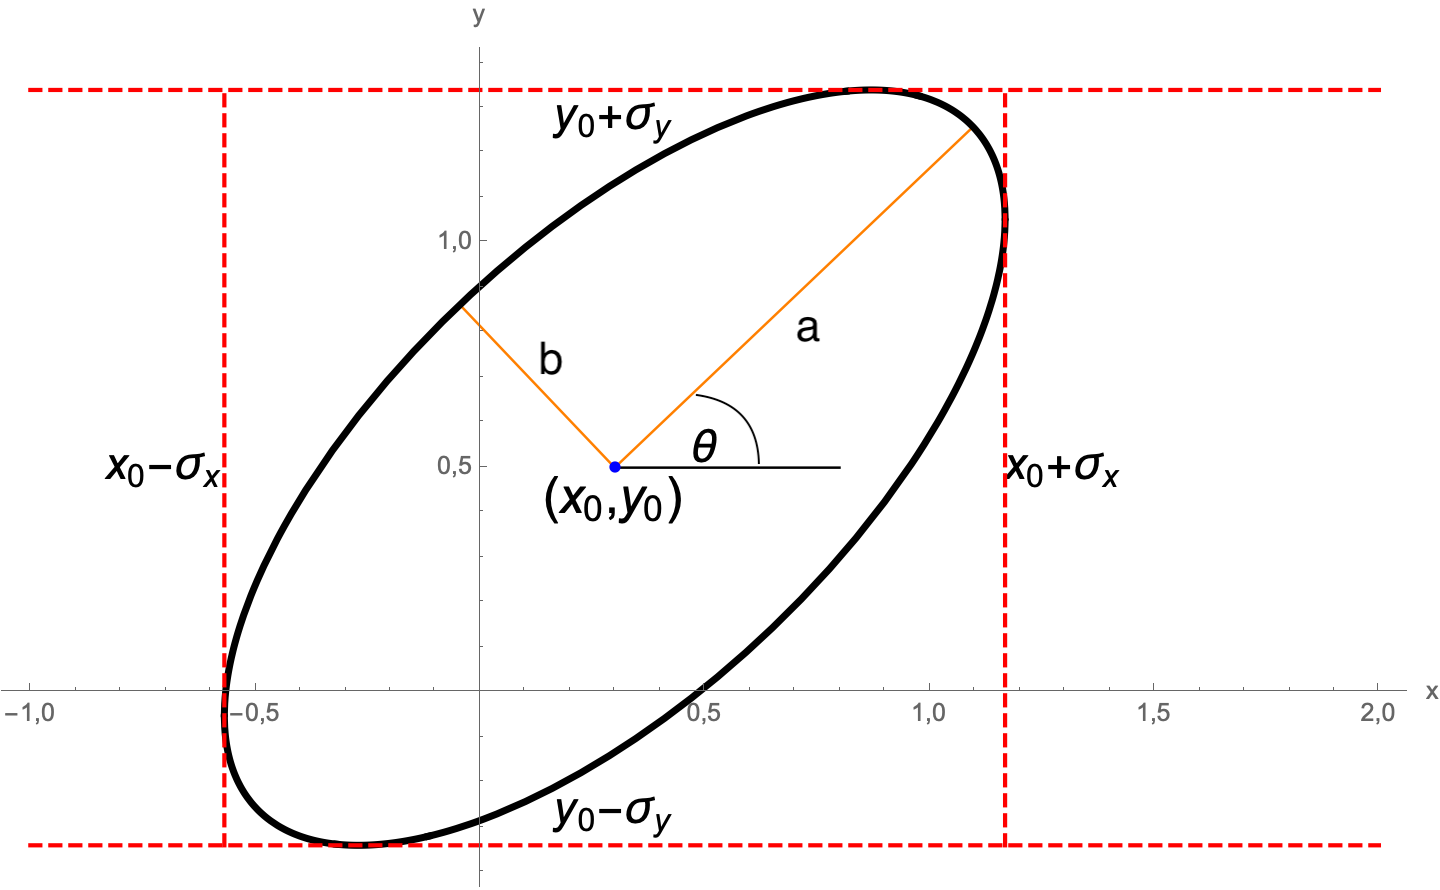
\includegraphics[width=0.6\linewidth]{4_photonid/ffs/procedure/ellipse}
    \caption{Parameters of the most general case of an ellipse.}
    \label{fig:ellipse_formulae:ellipse}
\end{figure}
